


\begin{figure}
\centering

\begin{tikzpicture}[->,>=stealth',shorten >=1pt,auto,node distance=5cm,
  thick,main node/.style={fill=white!20,draw,font=\sffamily\small\bfseries}]

  \node[main node] (vis) [text width=3cm] {Object Tracking};
  \node[main node] (ref) [below=1.0cm of vis] {Desired Position};
  \node[main node] (ik) [right=2.0cm of ref] {Walking Planner};
  \node[main node] (filter) [right=2.0cm of ik] {Filter};
  \node[main node] (hubo-ach) [below=1.0cm of filter] {Hubo-Ach};
  \node[main node] (hubo) [right=2.0cm of hubo-ach] {Hubo};



  \path[->, every node/.style={font=\sffamily\small}]
    (ref) edge node [above] {$(\theta_e, X_e)$} (ik);
%%    (ref) edge node [below] {$(\alpha,\beta,\gamma)$} (ik);
%  \path[->, every node/.style={font=\sffamily\small}]
%    (ref) edge node [below] {$(\alpha,\beta,\gamma)$} (ik);

 
  \path[->,every node/.style={font=\sffamily\small}]
    (vis) edge node [right] {$(x,y,z)$} (ref);

  \path[->,every node/.style={font=\sffamily\small}]
    (ik) edge node [above] {$\overline{\theta_d}$} (filter);

 \draw[->] ([xshift=-0.5 cm]filter.south)  -- node [left] {$\overline{\theta_r}$} ([xshift=-0.5 cm]hubo-ach.north)  ;
 \draw[->] ([xshift=0.5 cm]hubo-ach.north) -- node [left] {$\overline{\theta_a}$} ([xshift=0.5 cm]filter.south)  ;

 \path[<->,dashed, every node/.style={font=\sffamily\small}]
    (hubo) edge node [above] {CAN} (hubo-ach);
    
    
    \draw[->] ([yshift=0.0cm] hubo.north)  to [out=90,in=0] node [above] {RGB-D Camera} ([yshift=0.0cm] vis.east)  ;

%  \path[->,every node/.style={font=\sffamily\small}]
%    (hubo-ach) edge node [left] {$\theta_r$} (filter);

%  \path[->,every node/.style={font=\sffamily\small}]
%    (filter) edge node [right] {$\theta_a$} (hubo-ach);




% look into this and add z^-1

%\path [every node/.style={draw,minimum width=3cm, minimum height=5cm]}]
%  node (a) at (0,0) {}
%  [xshift=7cm]
%  node (b) at (0,0) {}
%  [xshift=7cm]
%  node (c) at (0,0) {};

%\begin{scope}[->,>=latex]
%    \foreach \i in {-2,...,2}{% 
%      \draw[->] ([yshift=\i * 0.8 cm]a.east) -- ([yshift=\i * 0.8 cm]b.west) ;}

%    \foreach \i in {1,2}{% 
%      \draw[->] ([yshift=\i * 0.8 cm]a.east) to [out=50,in=130] ([yshift=\i * 0.8 cm]c.west) ;} 

%    \foreach \i in {-1,-2}{% 
%      \draw[->] ([yshift=\i * 0.8 cm]a.east) to [out=-50,in=-130] ([yshift=\i * 0.8 cm]c.west) ;}
%\end{scope}


\end{tikzpicture}
\caption{The $(x,y,z)$ work space position of the objet is found via HSV tracking.  The rotation error $\theta_e$ and distance of the object from the projection of the robot onto the ground $X_e$ is sent to the \textit{walking planner}.  The walking planner decides if it has to turn or walk forwards. The robot will stop when it is within $0.2~m$ of the object and facing it within an error of $\pm 0.02~rad$.}
\label{fig:hubo-ach-walkingVservoing}
\end{figure}



Using a the well know HSV (Hue Saturation Value) tracking algorithm.  
HSV tracking was implemented via the use of built in libraries in OpenCV\cite{opencv}.

Fig.~\ref{fig:hubo-ach-walkingVservoing} shows the block diagram of the full system. 
The $(x,y,z)$ work space position of the objet is found via HSV tracking.  
The rotation error $\theta_e$ and distance of the object from the projection of the robot onto the ground $X_e$ is sent to the \textit{walking planner}.  
The walking planner decides if it has to turn or walk forwards. 
The robot will stop when it is within $0.2~m$ of the object and facing it within an error of $\pm 0.02~rad$.
The \textit{walking planner} is a state machine with the following characteristics:

\begin{equation}
f(\theta_e,X_e) = \left\{
     \begin{array}{ccl}
       \theta_e > 0.3~rad  & THEN & turn~0.3~rad\\
       \hline
       \theta_e < -0.3 & THEN & turn~-0.3~rad\\
       \hline
       0.3~rad > \theta_e > 0.02~rad && \\
       OR & THEN & turn~\theta_e~rad\\ 
       -0.02 < \theta_e < -0.3~rad & & \\
       \hline
        -0.02 < \theta_e < 0.02~rad &  &\\
        AND & THEN & step~forward~0.1~m\\
         X_e > 0.2~m &  &  \\
         \hline
        else & THEN & stop
     \end{array}
   \right.
\end{equation}



\begin{figure}[thpb]
  \centering
      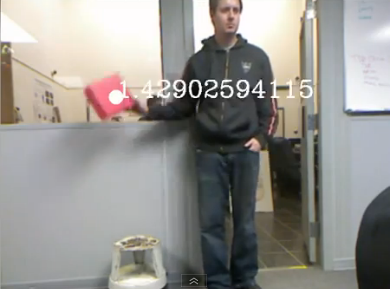
\includegraphics[width=0.69\columnwidth]{./examples/pix/hsv.png}
      
\includegraphics[width=0.3\columnwidth]{./qrcode/qrcode-hsvtrackingexample.png}\\
      Video: http://danlofaro.com/phd/tracking/\#HsvTracking
\caption{3D Object tracking using HSV color matching and an RGB-D camera to gain depth information.}
\label{fig:visualservoing}
\end{figure}
